In order to address the problem raised by Herley, 
we shall define how to distinguish between a secure and an insecure system.
While most of the literature (and this paper so far) have
correlated the problem of in-security to the maliciousness of
agents interacting with the system, we show that security
doesn't seem to stem from a malicious nature but, rather, insecurity 
raises from the lack of well-defined security requirements for the
design process of a system. We argue that the high number
of security vulnerability reported today are simply the realization
of potential system configurations, which deviate from the nominal
behavior just because the \emph{intended behavior}\fixnote{mr}{maybe ``nominal'' instead of ``intended'' is better and behavior can be confused with the
relation between assertions and beliefs which is not what we mean} of the system is not precisely 
defined in the specification at the very early stages of the engineering process. 
A reference engineering process (so called, system security lifecycle of a product)
is described, in details, in Section~\ref{sec:process}. However,
for the sake of simplicity, the reader can assume for this section that 
we are currently dealing with just the relation between 
the specification of a system and its design.

Given that we apply our theory to \emph{systems engineering} and that
the two foundational processes (exploitation and hacking) are based on the
concept of a system, we shall begin by defining what a system is, in its
abstract form.

\subsection{A Reference Model for Cybersecurity Engineering}\label{sec:vmodel}

\subsection{Abstract System State}\label{sec:systemstate}
The ISO/IEC/IEEE 15288:2015 (System Life Cycle Processes) provides a definition
of system as ``A combination of interacting elements organized to achieve one
or more stated purposes.''\autocite{ISO201515288}.  Therefore, a system can be
considered as a single agent where its interacting elements are the
constituents of the agent itself. For the sake of simplicity we first define a
system as an agent and then extend the definition to a ``combination of
interacting'' agents.  We use the same process of \autocite{Santaca2016abf} but
over slightly different terms. The differences and commonalities with
\autocite{Santaca2016abf} are described in Appendix~\ref{app:abf}. 

There is no agreement between the research communities (e.g.
Multi-Agent-System, Epistemic Logic) on which are the constituent of an agent
as a system. However, the same ideas revolved around for thousands of years.
Some relevant examples for our objective are the following.
\begin{itemize}
	\item In \autocite{Hintikka1962knowledge}, Hintikka describes the
		difference between Knowledge and Belief (as epistemological
		concepts), and the whole Doxastic logic defines in details how
		Beliefs can be formalized.
	\item In \autocite{Hintikka1993Information}, Hintikka describes the concept
		of Information and the difference with Knowledge and Belief.
	\item In \autocite{Empiricus1990Pyrrhonism}, the author states: ``The
		logical criterion also may be used in three senses -- of the
		agent, or the instrument, or the ``according to what''; the
		agent, for instance, may be a man, the instrument either sense
		perception or intelligence, and the ``according to what'' the
		application of the impression ``according to'' which the man
		proceeds to judge by means of one of the aforesaid
		instruments.'' 
	\item In \autocite{Santaca2016abf}, the authors defines an agent as a
		tuple of Assertions, Beliefs, and Facts.
\end{itemize}

If we consider \autocite{Empiricus1990Pyrrhonism}, the author applies a
``logical criterion'' to an agent, for instance a man, for instance a device in
a system (or a system) as in \autocite{Santaca2016abf}.  The instrument identified is sense
perception, because a man is considered as example, but we can abstract from the
concept of instrument and consider any received information, where information is
considered as in \autocite{Hintikka1993Information}; which can be
summarized by the following axiom: ``Information is specified by specifying
which alternatives concerning the reality it admits and which alternatives
excludes''. This means, for our argument, that considering a propositional
variable, which admits the two alternatives True/False, its information is
defined as Believed to be True/False and not Believed to be the opposite. 
%Similarly, when reasoning on a
%mereotopological region w.r.t. the RCC (e.g. RCC3 admits two regions to be
%equal, disjoint, or overlapping) information on this region should exclude
%some of the alternatives. 
Finally, in \autocite{Empiricus1990Pyrrhonism}
the author states that the logical criterium can be judged according to a frame of reference.
For our argument, as in \autocite{Santaca2016abf}, we define this concept
as Knowledge (or Facts); where knowledge is defined, as in \autocite{Steup2020epistemology}, as
a set of proposition known by an agent, such that: (i) knowledge requires belief,
(ii) knowledge require truth, (iii) knowledge must be \emph{properly justified}.

Before detailing what ``properly justified'' means, we discuss the mentioned
relation between agent and belief and we introduce a more formal definition
of knowledge and belief. For our argument, the only objective of
Information is to exchange beliefs between agents.
Due to the definition of Information and then with its relation to the probabilistic
correlation to truth/reality, we consider
information in relation with an agent's beliefs. Similarly, we consider
beliefs to define the actual behavior of an agent or a system. On the other hand,
Knowledge drives the nominal behavior of an agent or a system. This view
is not considered in most (if not all) the approaches to protocol verification
and the Dolev-Yao theory is usually applied to a representation/abstraction
of a protocol that only considers knowledge and transfer of knowledge (i.e.
if an agent sends a message, the recipient knows that message). However,
the security of a system is tightly related to the difference between
the nominal behavior and the actual (e.g. the implemented) one.

\begin{definition}{\bf System State and State-Space --}\label{def:system}
	The state of a system (or a sub-system) $s$ is identified with an
	instance of an agent state (see Definition~\ref{def:agent}) such that
	$s=\langle\rcc(\knowledgeRegion,\beliefRegion),\rcc(\knowledgeRegion,\informationRegion),\rcc(\beliefRegion,\informationRegion)\rangle$,
	where $\knowledgeRegion,\beliefRegion,\informationRegion$ are Regions
	of Knowledge, Beliefs, and Information respectively, and $\rcc$ is a
	specific relation between the Regions it predicates on.  The
	state-space of a system is then defined by the different $\rcc$
	relations between the three pairs of Regions defining the system and
	all the sub-systems.
\end{definition}
Therefore, a system state space can be seen as a superposition of multiple agent states where knowledge,
beliefs, and information are related between each other (in a mereotopological
space) through all the admissible RCC relations. 
\fixnote{mr}{are the next lines redundant?}A \emph{system state} (as an instance of the system state space)
is a specific configuration of
the $\rcc$ relations between the three regions. Therefore, a collection of 
system states defines a collection of choices for those $\rcc$ relations.

% \item  ``normally concern the state or the history of the entire universe but only
% of some small part of
% it''.  
% \item  ``Information and probability are inversely related'', i.e. ``
% the more alternatives a proposition admits of, the more probable and the less
% informative it is, and vice versa''

\begin{figure}[t]
	\centering
	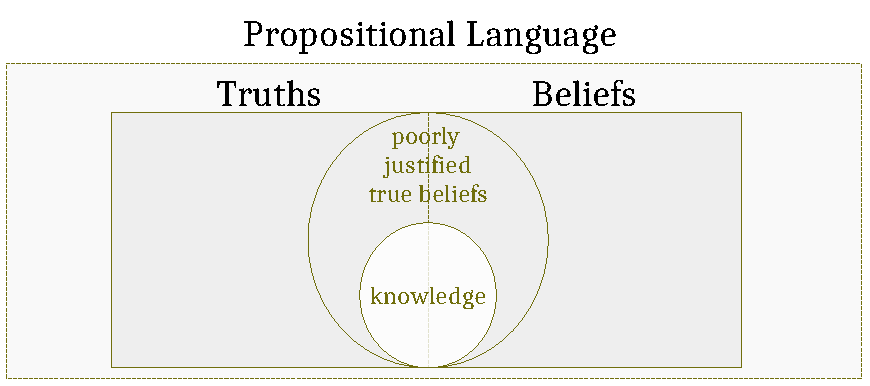
\includegraphics[width=.8\textwidth]{knowledge-belief.pdf}
	\caption{Informal representation of Knowledge and Belief}
	\label{fig:knowledge-belief}
\end{figure}

The difference between Knowledge and Belief is depicted in
Figure~\ref{fig:knowledge-belief} (see \autocite{wiki-knowledgebelief}).  However,
according to\autocite{Gettier2012knowledge},
Knowledge\footnote{``\emph{Theaetetus}: [\ldots] He said that knowledge was
true opinion accompanied by reason, but that unreasoning true opinion was
outside of the sphere of knowledge; and matters of which there is not a
rational explanation are unknowable -- yes, that is what he called them -- and
those of which there is are knowable. [\ldots] \emph{Socrates}: [\ldots] the
primary elements of which we and all else are composed admit of no rational
explanation; for each alone by itself can only be named, and no qualification
can be added, neither that it is nor that it is not, for that would at once be
adding to it existence or non-existence, whereas we must add nothing to it, if
we are to speak of that itself alone.  [\ldots]'' Plato -- Theaetetus 201
\autocite{Plato1914Plato}} as an epistemological concept is difficult to formally define. 
Similarly for the concept of information, Hintikka in \autocite{Hintikka1993Information}
states that ``A purely logical definition of information is impossible''.
In this work, however, we are not interested in how knowledge, information, or
belief can be precisely formalized from an epistemic standpoint.  We assume
that a semantic of a correct (i.e. commonly believed to be true) definition of epistemic knowledge exists, for
example the one given in\autocite{Hintikka1962knowledge} by Hintikka, and we
then define knowledge in terms of the Kripke structure defined in
Definition~\ref{def:modallogic}; similarly for Belief.

\begin{definition}{\bf Knowledge --}\label{def:knowledge}
Given an abstract collection of Agents $Ag$, and the modal operator
	$\knows{a}{}$ (where $a\in Ag$), Knowledge is defined as a region 
	of predicates known by an agent $\knowledge{a}=\bigcup_\Phi \knows{a}{\varphi}$ 
	(where $\Phi$ is the collection of all the propositions known by $a$).
	Given a proposition $P$, we extend the semantics of the Causality structure with:
	\begin{enumerate}[noitemsep]
		\item[$(\interpretation16)$] $\world\models\knows{a}{P}$ iff
			$\world'\models P$ for all $\world'$ such that
			$\world\modalrelation\world'$.
	\end{enumerate}
\end{definition}

\begin{definition}{\bf Belief --}\label{def:belief}
	Given an abstract collection of Agents $Ag$, and the modal operator
	$\believe{a}{}$ (where $a\in Ag$), Belief is defined as a region 
	of predicates believed by an agent $\belief{a}=\bigcup_\Phi \believe{a}{\varphi}$
	(where $\Phi$ is the collection of all the propositions believed by $a$).
	Given a proposition $P$, we extend the semantics of the Causality structure with:
	\begin{enumerate}[noitemsep]
		\item[$(\interpretation17)$] $\world\models\believe{a}{P}$ iff
			$\world\models\neg\knows{a}{\neg P}$ (i.e. the agent $a$ considers $P$ possible) 
			and $\world'\models P$ for all
			$\world'$ such that $\world\modalrelation\world'$.
	\end{enumerate}
\end{definition}

\begin{definition}{\bf Information --}\label{def:information}
	Given an abstract collection of Agents $Ag$, and the modal operator
	$\informs{a}{}$ (where $a\in Ag$), Information is defined as a region 
	of beliefs asserted by an agents $a$.
	%and transferred from $a$ to $b$ ($a\rightarrow b$).
	$\information{a}=\bigcup_\Phi \informs{a}{}{\varphi}$
	(where $\Phi$ is the region of all the propositions believed and asserted by $a$).
	Given a proposition $P$, we extend the semantics of the Causality structure with:
	\begin{enumerate}[noitemsep]
		\item[$(\interpretation18)$] $\world\models\informs{a}{P}$ iff
			$\world\models\belief{a}{P}$ (i.e. the agent $a$ considers $P$ possible), 
			$\world\models\neg\belief{a}{\neg P}$%, 
			%and $\world'\models P$ for all
			%$\world'$ such that $\world\modalrelation\world'$.
	\end{enumerate}
\end{definition}

\subsection{Operational System State}\label{sec:engsystemstate}
When dealing with a specification of a system (i.e. the design if the system
for a specific operation (as a generic operating/operational system),
considering abstract and general concepts such as knowledge, belief, or
information may result to be too abstract for the objectives of the overall engineering
process (e.g. verification and validation).
As an example, we are usually not
interested in information in abstract but to the transfer of that
information, which we call Assertions, made by a subset of agents. 
Therefore, we now define how we consider an agent for the engineering
of CPS.

\begin{enumerate}
	\item We consider Information only when the intention of exchanging 
		that Information is from a sender to 
		recipient is defined; and we call it \emph{Assertion}  
	\item Similarly, the portion of Beliefs we consider for system
		engineering is the one that builds (input) or describes
		(output) the behavior of an agent (strategy rules
		\footnote{``The logical structure of information is one of the
		most basic and one of the most basic and one of the simplest
		thing in the wide and wonderful world of logical analysis. This
		point can be put in a deeper perspective. A distinction
		[\ldots] ought to be made [--] between two kinds of rules (or
		principles) in any strategic activity like knowledge seeking.
		On the one hand you have the rules that define the game, e.g.
		how chessmen are moved on a board. The can be called
		\emph{definitory} rules.  They must be distinguished from rules
		[\ldots] that deal with what is better and what is worse in the
		game in question.  Definitory rules do not say anything about
		this subject. Rules which do can be called \emph{strategic
		rules}'' -- Hintikka in \autocite{Hintikka1993Information}}),
		and
	\item We consider a set of axiomatic \emph{Facts} (definitory rules) instead
		of considering the more general epistemic definition of
		Knowledge. Specifically, Facts describes:
		\begin{itemize}
			\item The functional architecture of each agents
			\item The physical/structural (HW/SW) architecture of each
				subsystem of agents and agent within a
				subsystem
			\item Other important aspects of the system that we
				describe afterwards in this paper, such as
				the assets and security properties 
		\end{itemize}
\end{enumerate}
We give a graphical representation of (sub-)system and agent in Figure~\ref{fig:system-agent}.

We note here (and describe with more details afterwards in this paper) that the
data flow can be defined as a transfer of Beliefs through Assertions (i.e. the
Beliefs flow).

\begin{figure}[t]
	\centering
	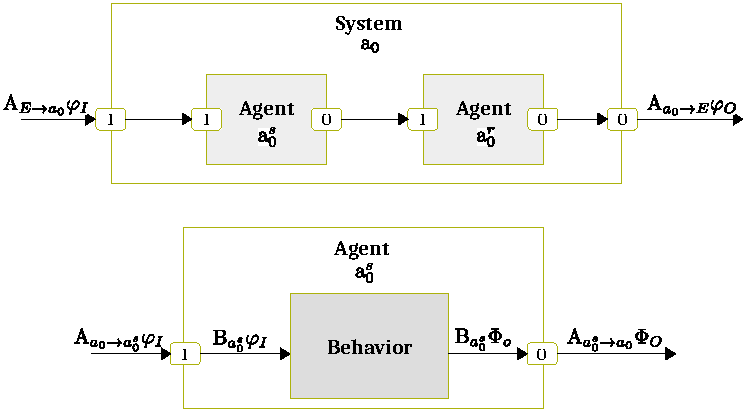
\includegraphics[width=.9\textwidth]{system-agent.pdf}
	\caption{Example of system and agent structure}
	\label{fig:system-agent}
\end{figure}

\begin{definition}{\bf Assertion -- }\label{def:assertion}
	An assertion is an intended transfer of beliefs between
	two agents $a$ and $b$ such that
	\begin{enumerate}[noitemsep]
		\item[$(\interpretation19)$] $\world\models\rassert{a}{b}{P}$ iff
			$\world\models\belief{a}{P}$, 
			$\world\models\neg\belief{a}{\neg P}$, 
			$\world'\models\rcc(\belief{a}{P},\belief{b}{P})$, 
			for all $\world'$ such that $\world\modalrelation\world'$.
	\end{enumerate}
\end{definition}

\begin{definition}{\bf Behavior -- }\label{def:behavior}
	The behavior of an agent is defined as the transformation process (e.g. defined as a
	protocol, or a functional architecture) that determines the
	output-beliefs based on input-beliefs and vice versa (where input-beliefs and
	output-beliefs are beliefs taken as input or output respectively).
	\begin{enumerate}[noitemsep]
		\item[$(\interpretation20)$] $\world\models\bigcup_{\Phi}\believe{s}{\varphi}$ and $\world\models\behave{a}{[\bigcup_{s\in S}\believe{s}{P_{s}}]}$ iff
			$\world\models\belief{a}{P'}$, 
			
		where $a$ is an agent, $S$ is a set of agents such that $a\neg\in S$, and the calculation of $P'$ is deteministic.
	\end{enumerate}
\end{definition}

\begin{definition}{\bf Fact -- }\label{def:fact}
Facts are a sub-region of Knowledge $\factRegion = \bigcup_\Phi \knows{a}{\varphi}$
	that predicate in a factive way, e.g.
	if $a$ knows that $P$ then $P$, and the region of facts is monotone (no revision).
	\begin{enumerate}[noitemsep]
		\item[$(\interpretation21)$] $\world\models\fact{a}{P}$ iff
			$\world \models \Box P$. 
	\end{enumerate}
\end{definition}

\begin{definition}{\bf Operational System State --}\label{def:system}
	An operational system (or a sub-system) is represented as an agent (see Definition~\ref{def:agent}) and then defined by the resulting state space,
	such that
	$s=\langle\rcc(\factRegion,\behaviorRegion),\rcc(\factRegion,\assertionRegion),\rcc(\behaviorRegion,\assertionRegion)\rangle$,
	where $\assertionRegion,\behaviorRegion,\factRegion$, are regions of assertions, behavior (i.e. the beliefs generated by the behavior), and facts respectively.
\end{definition}

As already presented in \autocite{Santaca2016abf} it follows that, defining
a system (or an operational system) with a fixed number of regions, there exist
an upper-bound to the number of possible configuration of a system, defined by
the possible relations between the different regions.
For completeness, we report in the next paragraph 
the calculation done in \autocite{Santaca2016abf}.

\Paragraph{Number of different configurations of a system}
The general formula to calculate the number of different types of agents is
$r^{\binom{n}{k}}$, where $r$ is the number of relations with arity $k$,
between $n$ different sets, where $r^e$ is the number of permutation of $r$
relations over $e$ elements with repetitions, with $e$ being the number of
$k$-ary combinations of $n$ sets, $\binom{n}{k}$.
In our case, $\binom{n}{k}=3$ since we consider $3$ sets
($\assertionRegion,\behaviorRegion,\factRegion$), and all the relations
considered in the RCC are binary.  Hence, using RCC5 (with five different
spatial relations) over three sets, we can theoretically define up to 125
different type of agents. However, only 54 of the 125 (as showed in
\cite{improvingRCC}) combinations are topologically correct with respect to
the definition of the relations of RCC5. Generalizing to all the RCCs:

\begin{itemize}%[nosep]
\item \emph{RCC3} --- theoretical: $3^3=27$,  correct: 15 
\item \emph{RCC5} --- theoretical: $5^3=125$, correct: 54
\item \emph{RCC8} --- theoretical: $8^3=512$, correct: 193
\end{itemize}

Hence, even if considering a different number of sets than the three
$\assertionRegion$, $\behaviorRegion$ and $\factRegion$ exponentially affects
the number of theoretical agents, the application of RCC downscales that number
of a factor that ranges from 1.8 to 2.5. In addition, using RCC5 we consider
3.6 times more (different) types of agents than RCC3, but using RCC8 would
allow us to consider 3.5 times more different agents.

In the quantitative evaluation of a single agent, depicted in Figure~\ref{fig:quantitative},
we argue that only 1 configuration represents the nominal (expected) behavior 
of the agent while the other configurations are either impossible to 
implement or diverge from the intended nominal behavior.

\begin{figure}[t]
	\centering
	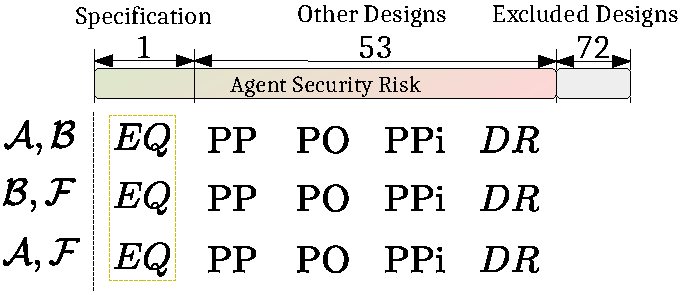
\includegraphics[width=.9\textwidth]{quantitative.pdf}
	\caption{Quantitative representation of the cybersecurity risk for a single agent}
	\label{fig:quantitative}
\end{figure}

As described beforehand in this section, the collection of Facts shall define
the functional and the physical architecture of an agent, but Assets and
security properties are defined as Facts. Given that understanding
why an Asset is considered as such by the user doesn't necessarily allow
us to better qualify an Asset, we consider the fact of ``being an asset'' as
a Boolean property of an Agent. 

\begin{definition}{\bf Asset --}\label{def:asset}
	\fix{mr}{asset def.}
\end{definition}

The definition of the security properties is given in Section~\ref{sec:properties}

\subsection{Qualitative Evaluation of Agent Space in $\abf$}\label{sec:agentspace}
While a quantitative analysis reveals how many possible configurations of an
agent (i.e. a system) exist w.r.t. the $\abf$ theory (i.e. $54/125$ in RCC5), a
qualitative analysis of the different configurations describes
the configurations allowed by the $\abf$ theory, and how those configurations can be
categorized.  In Table~\ref{tab:5com} we provide the generic composition table
of RCC5 over 3 regions instantiated over $\abf$, which shows the whole state
space for a single agent. The color coding of the table represents the 
risk function as a risk matrix as we detail afterwards in this Section.

A detailed qualitative categorization of agents over a theory similar to the
$\abf$ theory presented in this article is described in
\autocite{Santaca2016abf} but the differences in the formalization and of the
application requires another in-depth analysis. As depicted in
Figure~\ref{fig:soundness}, the relation between Facts, and Assertions and Behavior
defines the soundness of the design (admissible configurations of Assertions,
Behaviors and, in turn, Beliefs) w.r.t. the specification (what the
specification mandates, such as by the nature of the physical/functional
architectural models). Similarly, the relation between Assertions and Behavior defines the
soundness of the functional architecture.
We categorize agents by first analyzing the relations
between each pair of Regions defining an agent (i.e. $\abf$), and then we
categorize the different agents as tuple of the three Regions.
For the sake of simplicity, soundness is opposed to non-soundness in the following, however,
with the RCC we consider different ``degrees'' of soundness. For example,
in RCC5, if we consider EQ between two Regions as representing soundness, DR over the same Regions
represents non-soundness while PP, PO, PPi represents the different degrees of soundness.

\begin{figure}[t]
	\centering
	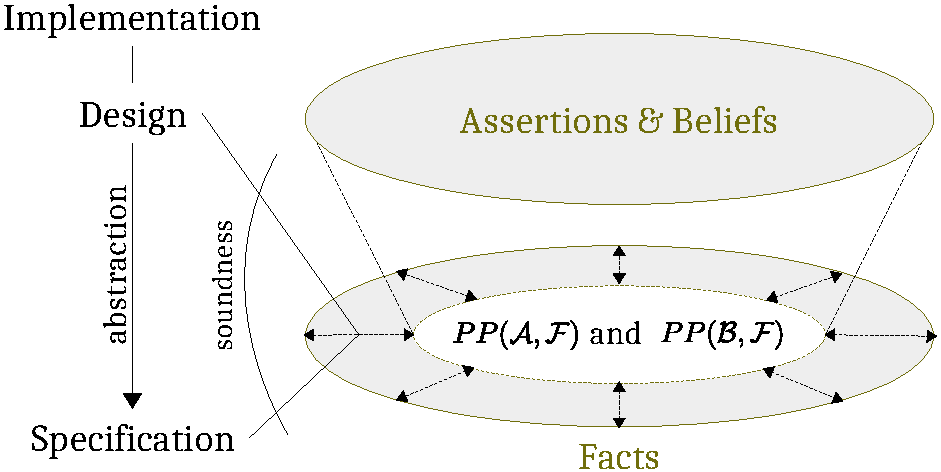
\includegraphics[width=.8\textwidth]{soundness.pdf}
	\caption{Example relation between Facts, and Assertions and Beliefs}
	\label{fig:soundness}
\end{figure}

\begin{enumerate}
	\item \Rcc{$\assertionRegion$}{$\behaviorRegion$}, in order to reason
		on the relation between assertions and behavior we first need
		to consider that, by definition, assertions are defined as
		transfer of information between two agents, e.g., $a$ and $b$.
		Therefore, as depicted in Figure~\ref{fig:system-agent}, an
		agent has two main categories of assertions, input and output assertions.
		Given an agent $a$ and a collection of asserted predicates
		$\Phi$, the Input assertions are those received
		by $a$ from an agent $s$ acting as a sender,
		$\rassert{s}{a}{\Phi}$; similarly, output assertions are sent
		from $a$ to a receiver $r$, $\rassert{a}{r}{\Phi}$. We shall consider
		two pairs of regions: 
		\begin{itemize}
			\item \Rcc{$\assertionRegion_{s\rightarrow
				a}$}{$\behaviorRegion$}, where the relation
				between Input-assertions and behavior describes
				the soundness of the execution of the
				functional architecture w.r.t. input
				elicitation. With more details, the ideal
				specification of the functional architecture,
				along with the expected inputs, defines the
				functional behavior of an ideal system.  If all
				the inputs (Assertions) are correctly handled
				in the functional specification (behavior) the
				specification is sound. 

			\item \Rcc{$\assertionRegion_{a\rightarrow
				r}$}{$\behaviorRegion$}, where the relation
				between behavior and outputs describes the
				completeness of the behavior defined in the
				specification w.r.t. the input elicitation.
				With more details, if all the outputs
				(assertions) of the functional architecture can
				be produced, the functional architecture is
				complete.
		\end{itemize}
	\item \Rcc{$\behaviorRegion$}{$\factRegion$} (Competence)
	\item \Rcc{$\assertionRegion$}{$\factRegion$} (Honesty)
\end{enumerate}

\Paragraph{Security Requirements} The following security requirement for a CPS specification can be summarized:
\begin{enumerate}
	\item Proper interaction between multiple correctly-behaving agents (in
		contrast with the ``Improper Interaction Between Multiple
		Correctly-Behaving Entities'' defined by the CWE in the
		categorization of ``research concepts'' in
		\autocite{MITRE2020CWEresearch}) is defined as $\eq{\assertionRegion}{\behaviorRegion}$
	\item The equality relation $\eq{\assertionRegion_{s\rightarrow a}}{\behaviorRegion}$
		describes the intended secure behavior as: the beliefs generated by the behavior of the functional architecture
		shall be complete w.r.t. the specified inputs of the agent. Therefore, \emph{the assertions received by an agent or a system
		shall be compliant with the expected inputs of the functional architecture}. For example, the inputs
		of the user of a SW must be sanitized to exclude deviations w.r.t. the expected inputs of the functions
		implemented in the SW. Another example is the type checking between allowed inputs and expected inputs.
\end{enumerate}

\begin{example}
	\begin{itemize}
		\item https://cwe.mitre.org/data/definitions/1000.html highlight diff between CWE ``improper interaction\ldots'' and our ''Proper interatcion\ldots'' and the internal categorization of the classes and base of the subitems of this CWE
	\end{itemize}
\end{example}

\begin{definition}{\bf Security and Insecurity of a System or an Agent --}\label{def:security}
\end{definition}

\begin{definition}{\bf Risk --}
\end{definition}
\begin{definition}{\bf Risk Matrix --}
\end{definition}

\begin{table}[t]
\centering
\begin{adjustbox}{width=\textwidth}
\begin{tabular}{r||c|c|c|c|c} 
& \dr{$\assertionRegion$}{$\behaviorRegion$} & 
	\po{$\assertionRegion$}{$\behaviorRegion$}& 
	\pp{$\assertionRegion$}{$\behaviorRegion$} &
	\ppi{$\assertionRegion$}{$\behaviorRegion$} & 
	\eq{$\assertionRegion$}{$\behaviorRegion$} \\
\hline
\hline %dr
 \multirow{3}{*}{\dr{$\behaviorRegion$}{$\factRegion$}} & 
	\cellcolor{abfred} & %dr
	\cellcolor{abf-rg-1}\dr{$\assertionRegion$}{$\factRegion$} & %po
	\cellcolor{abf-rg-2}\multirow{3}{*}{\dr{$\assertionRegion$}{$\factRegion$}} & %pp
	\cellcolor{abf-rg-3} \dr{$\assertionRegion$}{$\factRegion$}& % ppi
	 \cellcolor{abf-rg-4} \\ % eq
& \cellcolor{abfred}\all{$\assertionRegion$}{$\factRegion$}& %dr
	\cellcolor{abf-rg-1}\po{$\assertionRegion$}{$\factRegion$} & %po
	\cellcolor{abf-rg-2}\dr{$\assertionRegion$}{$\factRegion$} & %pp
	\cellcolor{abf-rg-3}\po{$\assertionRegion$}{$\factRegion$} & %ppi
	\cellcolor{abf-rg-4}\dr{$\assertionRegion$}{$\factRegion$}\\ % e q
 & \cellcolor{abfred}& %dr
	\cellcolor{abf-rg-1}\pp{$\assertionRegion$}{$\factRegion$} & %po
	\cellcolor{abf-rg-2}  & %pp
	\cellcolor{abf-rg-3}\pp{$\assertionRegion$}{$\factRegion$} & %ppi
	\cellcolor{abf-rg-4} \\ %eq
\hline %po
 \multirow{3}{*}{\po{$\behaviorRegion$}{$\factRegion$}} &
	\cellcolor{abf-rg-1}\dr{$\assertionRegion$}{$\factRegion$} & %dr
	\cellcolor{abf-rg-2} & %po
	\cellcolor{abf-rg-3}\dr{$\assertionRegion$}{$\factRegion$} & %pp
	\cellcolor{abf-rg-4}\po{$\assertionRegion$}{$\factRegion$} & %ppi
	\cellcolor{abf-rg-5} \\ %eq
 & \cellcolor{abf-rg-1}\po{$\assertionRegion$}{$\factRegion$} & %dr
	\cellcolor{abf-rg-2} \all{$\assertionRegion$}{$\factRegion$} & %po 
	\cellcolor{abf-rg-3}\po{$\assertionRegion$}{$\factRegion$} & %pp
	\cellcolor{abf-rg-4}\ppi{$\assertionRegion$}{$\factRegion$} & %ppi
	\cellcolor{abf-rg-5} \po{$\assertionRegion$}{$\factRegion$}\\%eq
 & \cellcolor{abf-rg-1}\pp{$\assertionRegion$}{$\factRegion$} & %dr
	\cellcolor{abf-rg-2} &  %po
	\cellcolor{abf-rg-3}\pp{$\assertionRegion$}{$\factRegion$} & %pp
	\cellcolor{abf-rg-4}& %ppi
	\cellcolor{abf-rg-5}\\ %eq
\hline %pp
 \multirow{4}{*}{\pp{$\behaviorRegion$}{$\factRegion$}} &
	\cellcolor{abf-rg-2}\dr{$\assertionRegion$}{$\factRegion$} & 
	\cellcolor{abf-rg-3}&
	\cellcolor{abf-rg-4} & %pp
	\cellcolor{abf-rg-5}\po{$\assertionRegion$}{$\factRegion$} & %ppi
	\cellcolor{abf-rg-6}\\ %eq
 & \cellcolor{abf-rg-2}\po{$\assertionRegion$}{$\factRegion$} & 
	\cellcolor{abf-rg-3}\po{$\assertionRegion$}{$\factRegion$} & 
	\cellcolor{abf-rg-4}\pp{$\assertionRegion$}{$\factRegion$} & %pp
	\cellcolor{abf-rg-5}\eq{$\assertionRegion$}{$\factRegion$} & %ppi
	\cellcolor{abf-rg-6}\pp{$\assertionRegion$}{$\factRegion$} \\ %eq
 & \cellcolor{abf-rg-2}\pp{$\assertionRegion$}{$\factRegion$} & 
	\cellcolor{abf-rg-3}\pp{$\assertionRegion$}{$\factRegion$} & 
	\cellcolor{abf-rg-4} & %pp
	\cellcolor{abf-rg-5}\pp{$\assertionRegion$}{$\factRegion$} & %ppi
	\cellcolor{abf-rg-6} \\ %eq
 & \cellcolor{abf-rg-2}&
 	\cellcolor{abf-rg-3} & 
	\cellcolor{abf-rg-4}& %pp
	\cellcolor{abf-rg-5}\ppi{$\assertionRegion$}{$\factRegion$} & %ppi
	\cellcolor{abf-rg-6} \\ %eq
\hline %ppi
 \multirow{3}{*}{\ppi{$\behaviorRegion$}{$\factRegion$}} &
 	\cellcolor{abf-rg-3}\multirow{3}{*}{} &
 	\cellcolor{abf-rg-4}\dr{$\assertionRegion$}{$\factRegion$} &
 	\cellcolor{abf-rg-5}& %pp
 	\cellcolor{abf-rg-6}& %ppi
 	\cellcolor{abf-rg-7} \\ %eq
& \cellcolor{abf-rg-3}\dr{$\assertionRegion$}{$\factRegion$} &
 	\cellcolor{abf-rg-4}\po{$\assertionRegion$}{$\factRegion$} & 
 	\cellcolor{abf-rg-5}\all{$\assertionRegion$}{$\factRegion$}& %pp
 	\cellcolor{abf-rg-6}\ppi{$\assertionRegion$}{$\factRegion$}& %ppi
 	\cellcolor{abf-rg-7}\ppi{$\assertionRegion$}{$\factRegion$}\\ %eq
& \cellcolor{abf-rg-3} & 
	\cellcolor{abf-rg-4}\ppi{$\assertionRegion$}{$\factRegion$} & 
	\cellcolor{abf-rg-5} & %pp
	\cellcolor{abf-rg-6}& %ppi
	\cellcolor{abf-rg-7}\\ %eq
\hline %eq
	\eq{$\assertionRegion$}{$\factRegion$} & 
	\cellcolor{abf-rg-4}\dr{$\assertionRegion$}{$\factRegion$} & 
	\cellcolor{abf-rg-5} \po{$\assertionRegion$}{$\factRegion$} & 
	\cellcolor{abf-rg-6}\pp{$\assertionRegion$}{$\factRegion$} & %pp
	\cellcolor{abf-rg-7} \ppi{$\assertionRegion$}{$\factRegion$} & %ppi 
	\cellcolor{abfgreen} \eq{$\assertionRegion$}{$\factRegion$}  %eq
\end{tabular}
\end{adjustbox}
\caption{RCC5 composition table over 3 regions. The results show that there
exist 54 possible relations and the coloring anticipates the ideal risk matrix
(green the secure state with low risk, red the high risk state, and a gradient
of medium risk states). 
\all{$\assertionRegion$}{$\factRegion$} = \{\dr{$\assertionRegion$}{$\factRegion$}, \po{$\assertionRegion$}{$\factRegion$}, \pp{$\assertionRegion$}{$\factRegion$}, \ppi{$\assertionRegion$}{$\factRegion$}, \eq{$\assertionRegion$}{$\factRegion$}\}
\label{tab:5com}}
\end{table}

\subsection{System Security Evolution}\label{sec:systemevoution}
\fix{mr}{
Facts should be correlated to the causality principle. Therefore a
specification in opnet should be translated into vmt and by bounded model
checking with nuxmv identify a path towards an undesired state, if that fails
use abf to mutate the first state into one of the possible according to abf and
re-run nuxmv.

Knowledge is the theory itself, an instance is the facts of a design of it. A
testing process tests facts against knowledge as much as we test a cps design
choices against its specification.  Information carries the knowledge of the
negation of the opposite of the information. Therefore an assertion carries the
belief (as a result of the behavior execution) of not the opposite. But, as
Hintikka States in "popper" our previous statement is true if the probability
distribution of the information is representative wrt the causality structure
(i.e. knowledge and facts, see email before). So, based on our theory, the
assertions should have a number between 3 to 5 possible negated meaning, one
per each rcc if reference and not just a negation of the information. Those
negation representative of an insecure configuration on the communication of
the system. In turn, those configurations should categorize all the CWE.  The
fact that weaknesses are generated by mankind but not exploited makes malicious
attacks confined to the hackers (and black-hat hackers). Fix: move black-hat
hackers as subregion of mankind with malicious intent. Describe the intent as a
desire of reaching a breach of a cybersecurity property over an asset (agent of
the system), instead of searching for a specific attack. The tool would then
translate the system from opnet to abf formula. The abf tool generates all the
sat state of the system fix: add state to all def before this text. And we
shall define the causality relation between the different states generated by
the abf tool as chosen nondeterministically from the possible sat states by a
model checker such as nuxmv.

By calculating sat instead of validity with abf tool and then adding it to the
causality structure of a system fact description, e.g. in nuxmv; we can
calculate a path for reachability of an insecurity property violated on an
agent which represents an asset. Whenever nuxmv fails, we can add a new state
and re-run the process. Those guesses should be better managed by a trained
v-ai since the inference by induction from the partial information of the
system in which we represent the assertions as negation of a beliefs and
without rcc do not carry enough information for a Reasoner that doesn't
implemented rcc.
}
